%!TEX root = main.tex

\newpage
\subsection{수식 작성하기}
\label{subsec:ams}
드디어 \lt 의 꽃, 수식에 대해 설명을 드릴 차례입니다.
다른 어떤 편집기보다도 강력하고 편리한 수식 편집 기능을 가지고 있는 \lt 인 만큼, 실질적으로 수식 편집의 표준으로 자리 잡았기 때문에 다양한 곳에서 이제 배우는 것들을 이용할 수 있을 겁니다.
역시나 예시부터 볼까요?

\begin{Verbatim}[frame=single]
\documentclass{article}
\usepackage{kotex}
\usepackage{setspace}
\usepackage{amsmath}
\usepackage{amssymb}
\usepackage[left=2.5cm,right=2.5cm,top=3cm,bottom=3cm,a4paper]{geometry}
\begin{document}
	\doublespacing
	\noindent 수식을 입력해 봅시다.\\
	막 내용을 입력하다 중간에 짧은 수식을 넣을 수 있습니다.\\
	예를 들어 $c \in A$ 이렇게 말입니다.\\
	조금 길거나 큰 수식을 따로 입력할 수도 있습니다.\\
	예를 들어
	\[\left\{ \begin{array}{ll}
		a \in f(a)\\
		a \notin f(a)
	\end{array} \right.\]
	이렇게 말입니다.\\
	심지어
	\begin{align}
		|f(x)|=|sf_1(x)+tf_2(x)| &\le |sf_1(x)|+|tf_2(x)| \nonumber
		\\&=|s||f_1(x)|+|t||f_2(x)| \nonumber
		\\&\le |s|c_1|g(x)|+|t|c_2|g(x)| \nonumber
		\\&=(|s|c_1+|t|c_2)|g(x)| \nonumber
	\end{align}
	이런 것도 됩니다.\\
	\LaTeX 은 정말 많은 수식 요소들을 지원해줍니다.\\
	$a^{bcd}_{efg}$와 같은 첨자는 물론이고, $\sum$, $\int$같은 것도 지원합니다.
	\[\frac{\pi}{2}\]
	이렇게 분수도 잘 됩니다.
\end{document}
\end{Verbatim}
역시 바로 다음 페이지에서 결과물을 확인하실 수 있습니다.

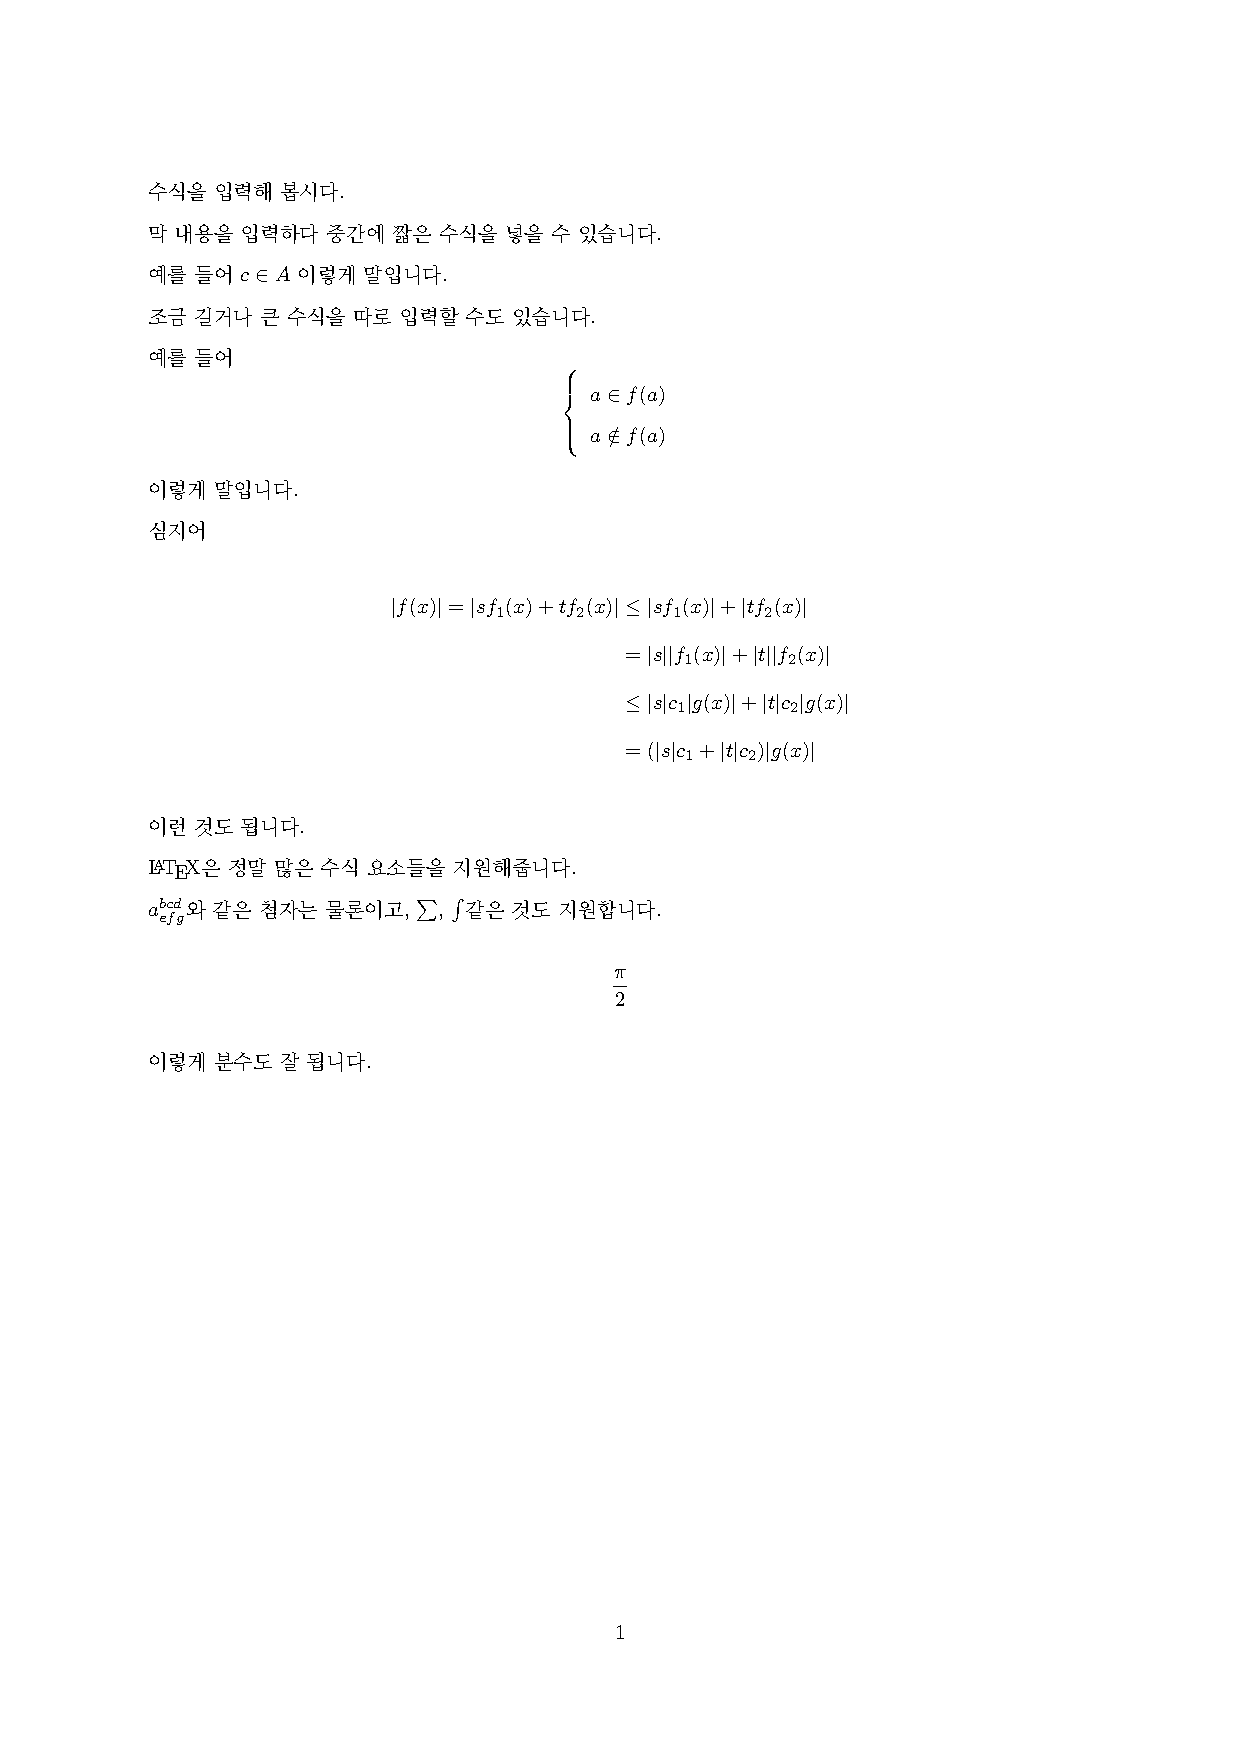
\includepdf[fitpaper=true]{example/mathexamplepdf.pdf}

예시를 잘 보면서, 천천히 시작부터 보도록 합시다.

\subsubsection{패키지 사용하기}
\label{subsec:ams-package}
보통 수식을 제대로 입력하려면 두 가지 package를 사용해야 합니다.
amsmath와 amssymb이 바로 그것들입니다.
수식을 입력해야 하는 문서라면 \verb|\usepackage{amsmath}|와 \verb|\usepackage{amssymb}|을 preamble에 입력해주세요.
참고로 한 번에 \verb|\usepackage{amsmath, amssymb}|라 쓸 수 있습니다.
수식은 웬만한 문서에 들어가기 때문에 이 한 줄을 기본적으로 입력해 두는 것을 추천합니다.
패키지를 불러왔다면, 이제 문서 어디든 수식을 입력할 준비가 된 것입니다.

\subsubsection{입력 시작하기}
\label{subsec:ams-start}
\lt 에서 수식을 입력하기 위해서는 따로 수식 편집기를 킨다거나, 그림을 추가하듯 추가하는 것이 아니라 기호 또는 command를 통해 수식을 입력함을 표시하면 됩니다.
그 방식에는 크게 세 가지 정도가 있습니다.

\paragraph{짧은 수식 삽입하기}
길고 크고 엄청난 수식을 입력하는 것이 아니라면, 보통의 경우는 수식을 문장의 중간에 넣고 싶을 겁니다.
이 때에는 내용을 입력하다가 수식을 입력하고 싶을 때 \verb|$...$|를 이용하면 됩니다.
보통 수식에서 많이 쓰이는 기호들은 저 달러 표시 안에 있어야 \lt 에서 인식할 수 있습니다.
또 저 안에 있으면 글꼴 자체가 수식에 맞도록 바뀝니다.
이 외에도 사람이 보기 좋은 수식으로 알아서 맞추어 주도록 하는 마법의 기호입니다.
다만 조금 길거나 여러 줄로 넘어가는 수식은 입력하기 어렵습니다.
꼭 일반적인 문장 중간에 넣고 싶을 때 사용해주시기 바랍니다.

\paragraph{긴 수식 삽입하기, 수식만 따로 삽입하기}
길고 크고 엄청난 수식을 입력하고 싶거나, 그래야 한다면 조금 다른 방법을 이용해야 합니다.
사실 정확히 말하자면 꼭 길지 않더라도 수식을 문장과 분리하여 따로 삽입하려면 이 방법을 이용해야 합니다.
바로 \verb|\[...\]|를 사용하는 겁니다.
이 안에 있는 모든 텍스트는 수식 입력으로 인식해서 수식으로 바꿔줍니다.
여러 행의 수식은 보통 이 방식으로 입력해줘야 하며 위의 방식보다 안정적으로 수식을 작성할 수 있습니다.
다만 이 방식 역시 모든 것이 가능한 것은 아닙니다.
그래도 웬만한 수식은 여기까지의 방법만 알아도 충분히 가능합니다.

\paragraph{특별한 수식들}
위 두 가지 방법이 아닌 다른 방법으로 수식을 입력하는 경우도 있습니다.
예시에서는 \verb|\begin{align}|이 이에 해당한다고 볼 수 있습니다.
\verb|\begin{align}|에 대한 자세한 설명은 뒤 \ref{subsec:ams-func}에서 하도록 하겠습니다.
이 외에도 \verb|\begin{equation}|, \verb|\begin{displaymath}| 등의 수식 환경을 이용할 수 있습니다.

\paragraph{}
세 가지 방법 중 상황에 맞게 한 가지를 골라 수식을 입력하기 시작하면 됩니다.

\subsubsection{다양한 기능}
\label{subsec:ams-func}
\lt 가 수식 입력에서 그렇게 두각을 나타내고 실질적인 업계 표준이 되어 다른 편집기가 베낄 정도로 뛰어난 이유는 위에서 말씀드렸던 입력의 용이성 외에도 수식에 필요한 기능을 거의 전부 가지고 있으며 이를 미려한 디자인으로 출력해준다는 것에 있습니다.
이제 그 많은 기능들 중 자주 필요로 하는 기능들 위주로 몇가지 소개해드리려 합니다.

\paragraph{빈칸 띄우기}
수식 모드에서 단순한 빈 칸과 줄바꿈은 적용되지 않습니다.
수식에서 모든 임의로 설정하지 않은 공백은 그 수식에 맞게 알아서 설정됩니다.
이 공백을 임의로 제어하기 위해서는  \verb|\,|, \verb|\quad| 또는 \verb|\qquad|와 같은 특별한 명령으로 지정해야 합니다.
자세한 정보는 표\ref{tab:quad}을 참조하세요.

\paragraph{글꼴 바꾸기}
수식 모드에서 모든 글자는 수식에 맞는 글꼴로 바뀌어 표현됩니다.
이 때문에 알파벳을 입력하면 이를 변수로 취급하여 변수 글꼴로 바꿔줍니다.
일반 텍스트를 수식 안에서 사용하고 싶다면 텍스트를 \verb|\textrm{...}| 안에 넣으면 됩니다.

\paragraph{벡터 표시, 밑줄 등 줄긋기}
벡터를 표시하거나 선분을 표시하는 등 글자 위에 줄을 긋거나 밑줄을 쳐야 할 때가 있습니다.
벡터는 \verb|\overrightarrow{...}|와 같은 식으로 표현할 수 있습니다.
\verb|\overline{...}|처럼 그냥 선 역시 그릴 수 있습니다.
자세한 것은 표 \ref{tab:overunder}를 확인해주세요.

\paragraph{열 맞춰 쓰기}
수식을 여러 행 쓰다보면 등호와 같이 열을 맞춰 쓰고 싶을 때가 있습니다.
\verb|\begin{align}|을 사용하면 열을 맞추어 쓰고 싶은 여러행 수식을 마치 표 작성하듯 쉽게 입력할 수 있습니다.
표 작성과 방식이 굉장히 비슷하기 때문에, \ref{subsec:tabfig}를 미리 보고 익히셔도 좋습니다.
방식을 설명해드리자면, 먼저 예시를 봅시다.
예시에서 볼 수 있듯 등호, 부등호 처럼 같은 열에 맞춰 쓰고 싶은 기호들 앞에 공통된 기호를 하나 입력했습니다.
\verb|&|입니다. 이 기호는 표에서도 비슷한 역할을 하므로 기억해 둡시다.
즉 같은 열에 맞추어 쓰고 싶은 부분 바로 앞에 \verb|&|를 붙이고, 줄바꿈은 아시는 대로 \verb|\\|를 이용하시면 됩니다.

\paragraph{여러 줄 묶기}
혹은 대괄호로 여러 행의 식을 묶어 표현해야 할 때도 있습니다.
여러 개의 식으로 정의되는 함수를 표현한다거나 할 때, 큰 중괄호로 식들을 묶는 방식을 많이 보셨죠?
바로 그것을 쉽게 표현할 수 있다는 겁니다.
예시에도 나와 있듯이 \verb|\[\]| 안에 \verb|\begin{array}{...}|를 이용하는 방법입니다.
이 환경 역시도 표 작성 방식과 거의 일치합니다.
구체적이고 자세한 것은 역시나 \ref{subsec:tabfig}를 먼저 읽어서 이해하시는 것을 추천드립니다.
간략히 설명을 드리자면, \dots 에는 묶고 싶은 수식의 열과 각 열의 정렬 방식에 따라 알맞은 문자를 넣습니다.
array 환경 앞에는 \verb|\left|, 그리고 중괄호와 같이 묶는 데 쓸 기호를 입력합니다.
array 환경 안에서 묶을 식들을 예시와 같이 입력하고, array 환경이 끝나고 \verb|\right.|을 입력하면 됩니다.

\subsection{표와 그림}
\label{subsec:tabfig}


%%% Local Variables:
%%% mode: latex
%%% TeX-master: "main"
%%% End:
